%-------------------------------------------------------------------------------
% yum_new_gui
%-------------------------------------------------------------------------------
%
% \file        yum_new_gui.tex
% \library     Documents
% \author      Will Godfrey
% \date        2021-7-21
% \version     $Revision$
% \license     $XPC_GPL_LICENSE$
%
%     Describes the changes in the GUI structure.
%
%-------------------------------------------------------------------------------

\section{Revised Graphical Interface}
\label{sec:revised_interface}
   When \textsl{Yoshimi} was forked from \textsl{ZynAddSubFX} all windows were of
   a fixed size. This perfectly suited the resolution of monitors that were
   available at the time, but as resolution increased over the years,
   \textsl{Yoshimi's} windows became progressively smaller. Eventually we were
   getting complaints about this. It came to head with the introduction of 4K
   screens. On such a display a magnifying glass was needed to read the text!

   FLTK 1.3.x has some resize capability and will keep the graphics mostly in
   scale, but not the text, nor things like tabs and menu bars. Therefore we had
   to develop work-arounds and emulations for these. Eventually the following
   decisions were made.
\begin{itemize}
   \item{All windows will be independently resizeable up to the full screen size.}
   \item{Windows and their contents will stay in scale.}
   \item{Inserts (such as Formant windows) from different sections will have
   their own set of positions/sizes.}
   \item{Last seen positions and sizes will be saved.}
   \item{Different \textsl{Yoshimi} instances will have their own set of
   positions/sizes.}
\end{itemize}

\pagebreak
   The first example shows Yoshimi with all visible windows at their default sizes
   on a 1920x1080 monitor. Notice the System Sends window (the smallest one)
   alongside the Main window.
\begin{figure}[H]
   \centering
   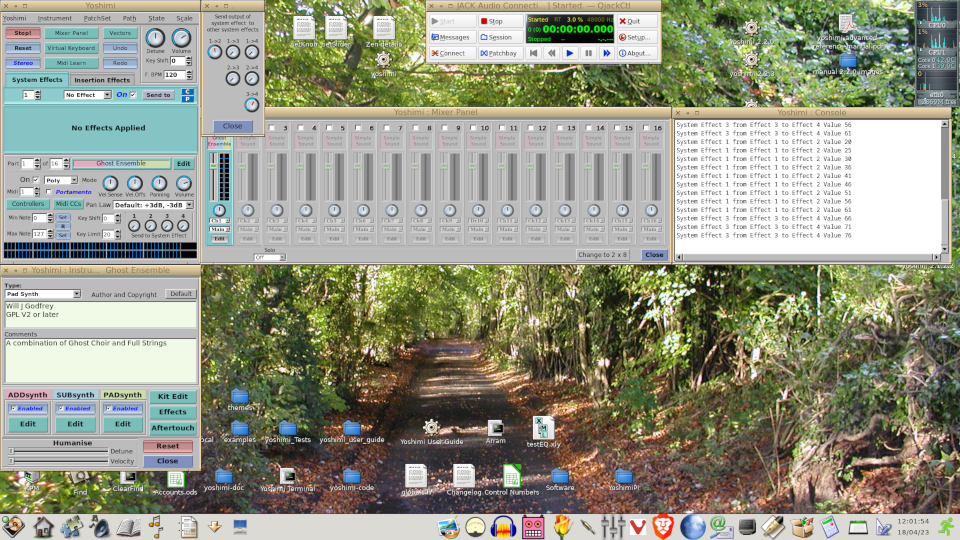
\includegraphics[scale=0.625]{2.1.0/gui_normal.png}
   \caption{Windows at default size}
   \label{fig:default_size_windows}
\end{figure}
   Next we show the same view, but with the System Sends window resized to the full
   height of the display. Notice that everything remains perfectly in scale.
\begin{figure}[H]
   \centering
   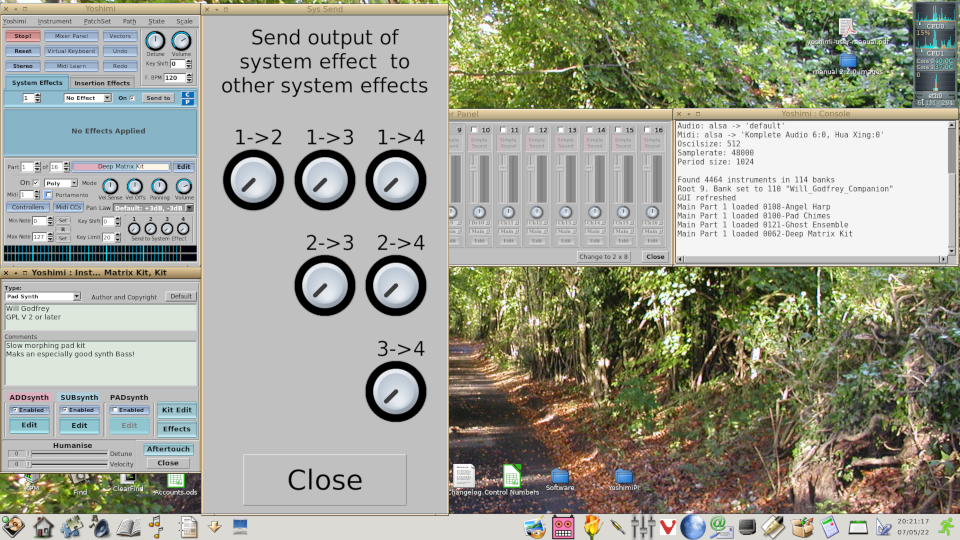
\includegraphics[scale=0.625]{2.1.0/gui_big.png}
   \caption{System Sends window resized}
   \label{fig:resized_sends_window}
\end{figure}
\subsection{Revised Graphical Interface / The Filer}
\label{subsec:interface_filer}
   One feature that proved impossible to work round was the default FLTK file
   chooser. The only recourse was to replace it with our own dedicated one. This
   actually gave us the opportunity to discard all generic features and controls,
   just providing exactly what \textsl{Yoshimi's} needed. This neatly fits with
   \textsl{Yoshimi's} uncluttered ethos of only showing you what you need to see.

   Below is a typical entry for loading a patchset.
\begin{figure}[H]
   \centering
   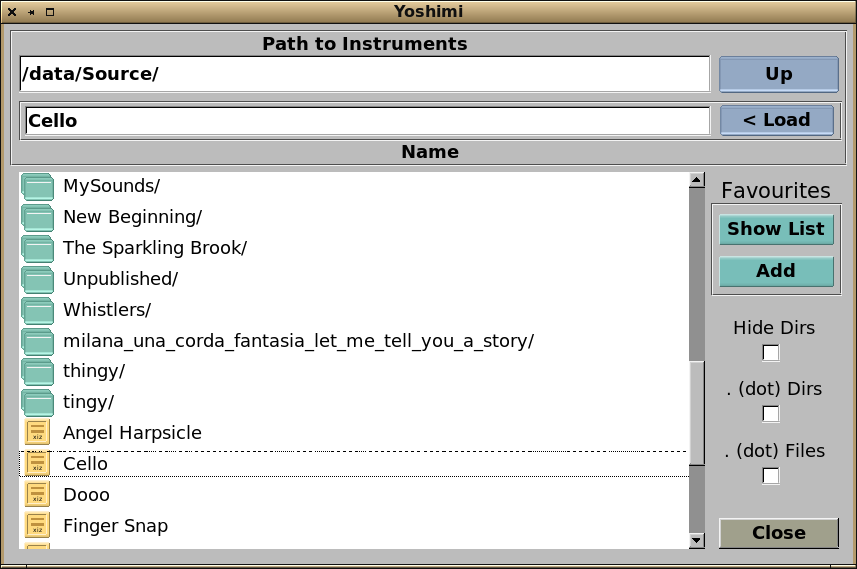
\includegraphics[scale=0.5]{2.1.0/filer.png}
   \caption{A filer 'Load' window}
   \label{fig:filer_load_window}
\end{figure}

When selecting 'Show Favourites, the existing filer window is overlaid with the
following view. Notice, it retains the path as a reminder.
\begin{figure}[H]
   \centering
   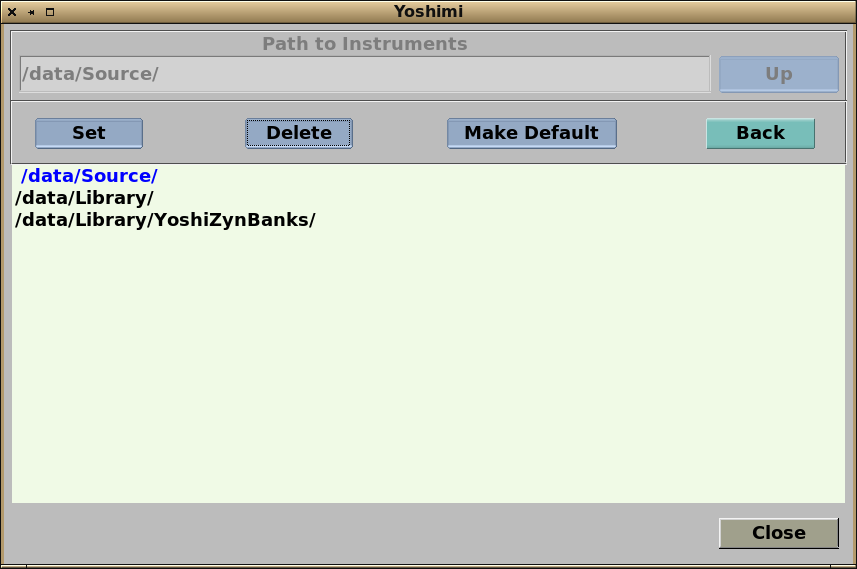
\includegraphics[scale=0.47]{2.1.0/favourites.png}
   \caption{The filer 'Favourites window}
   \label{fig:filer_favourites_window}
\end{figure}

%-------------------------------------------------------------------------------
% vim: ts=3 sw=3 et ft=tex
%-------------------------------------------------------------------------------
